\begin{figure}[t]
    \centering
    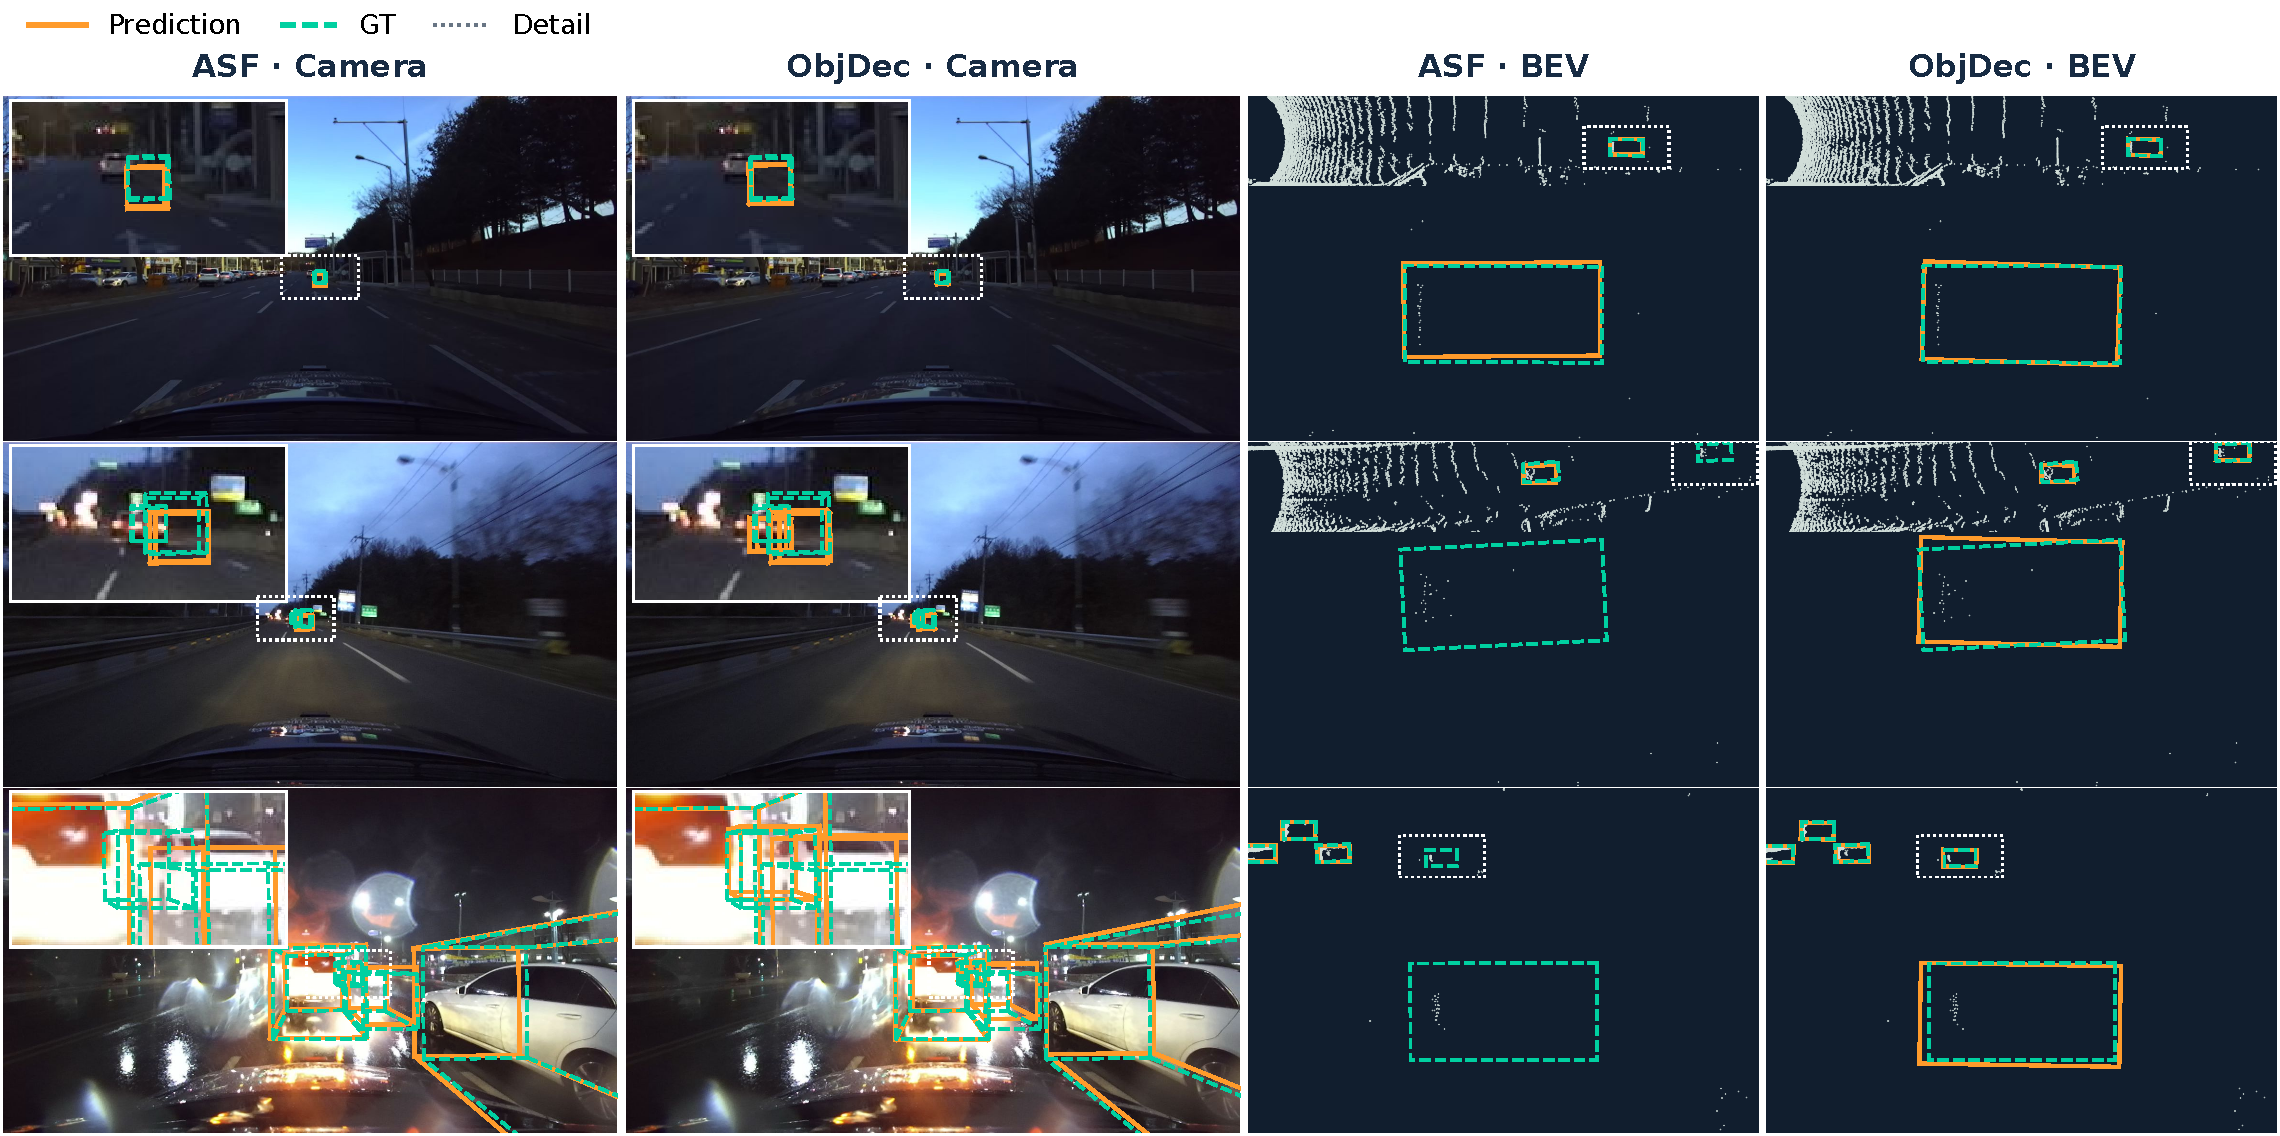
\includegraphics[width=\linewidth]{assets/figure5.pdf}
    \caption{Qualitative comparison of the released ASF checkpoint and ObjDec on identical K-Radar v1 test frames. The first two columns show calibrated camera projections with enlarged insets; the last two show full LiDAR BEV views above matched detail windows. Orange solid boxes denote Sedan predictions with scores above 0.3; green dashed boxes denote GT. Both methods use identical inputs, detection postprocessing, display thresholds, and camera/BEV crop windows. White dotted rectangles mark the enlarged regions. Full BEV views cover $x\in[0,72]$ m and $y\in[-6.4,6.4]$ m, while each detail window spans $12\times6$ m. For the highlighted GT, maximum 3D IoU among retained predictions changes from ASF to ObjDec as follows, from top to bottom: 0.572 to 0.719, 0.000 to 0.476, and 0.000 to 0.741. These values describe selected-object box overlap rather than AP; the middle example remains below IoU 0.5. Figure~\ref{fig:e3} includes an additional improvement and a localization counterexample.}
    \label{fig:e-comparison}
\end{figure}
